%!TEX root = ../template.tex
%%%%%%%%%%%%%%%%%%%%%%%%%%%%%%%%%%%%%%%%%%%%%%%%%%%%%%%%%%%%%%%%%%%%
%% chapter5.tex
%% NOVA thesis document file
%%
%% Chapter with lots of dummy text
%%%%%%%%%%%%%%%%%%%%%%%%%%%%%%%%%%%%%%%%%%%%%%%%%%%%%%%%%%%%%%%%%%%%

\typeout{NT FILE chapter5.tex}%

\chapter{Work Plan}
\label{cha:work_plan}

This chapter contains the planned progress, organized into distinct tasks, each with a description. Some tasks will be developed in parallel. 
Additionally, a Gantt chart is presented in Figure \ref{fig:gantt_chart} to illustrate the timeline for each task.

\begin{itemize}
    \item \textbf{Mockup Development}: This task focus developing a mockupthat includes map visualization within a \gls{VE}, along with the associated functionalities and \gls{3D} models visualization.
    \item \textbf{\gls{3D} Models \& Interaction}: This phase consists on the generation of \gls{3D} models using photogrammetry, and implementing user interactions with these models, such as applying filters, zooming, and scaling.  Initially, this phase will focus on a simulation involving a single object.
    \item \textbf{\gls{GIS} Implementation}: This task comprises the creation of a map that allows user interaction with \glspl{POI} represented by markers, integrating layers, and providing functionalities as outlined in Section \ref{sec:requirements}.
    \item \textbf{Database Creation for Repository}: In this phase, a database will be established to store important data, including artefacts and escavation metadata. The structure will initially focus on a single object, as proposed in Section \ref{sec:data_structure}.
    \item \textbf{\gls{VR} Integration}: This phase covers the development of \gls{VR} functionality in Unity, including its integration with the map and communication with users via web requests through the REST API.
    \item \textbf{Testing}: This task involves user testing of functionalities, usability and performance, including participation from VICARTE investigators.
    \item \textbf{System Evaluation}: Following the completion of the testing phase, the system evaluation process will begin. This phase will include user questionnaires and potential system improvements based on the feedback received. 
    \item \textbf{Documentation}: The dissertation report will be developed during the whole process.
\end{itemize}

\begin{figure}[h!]
    \centering
    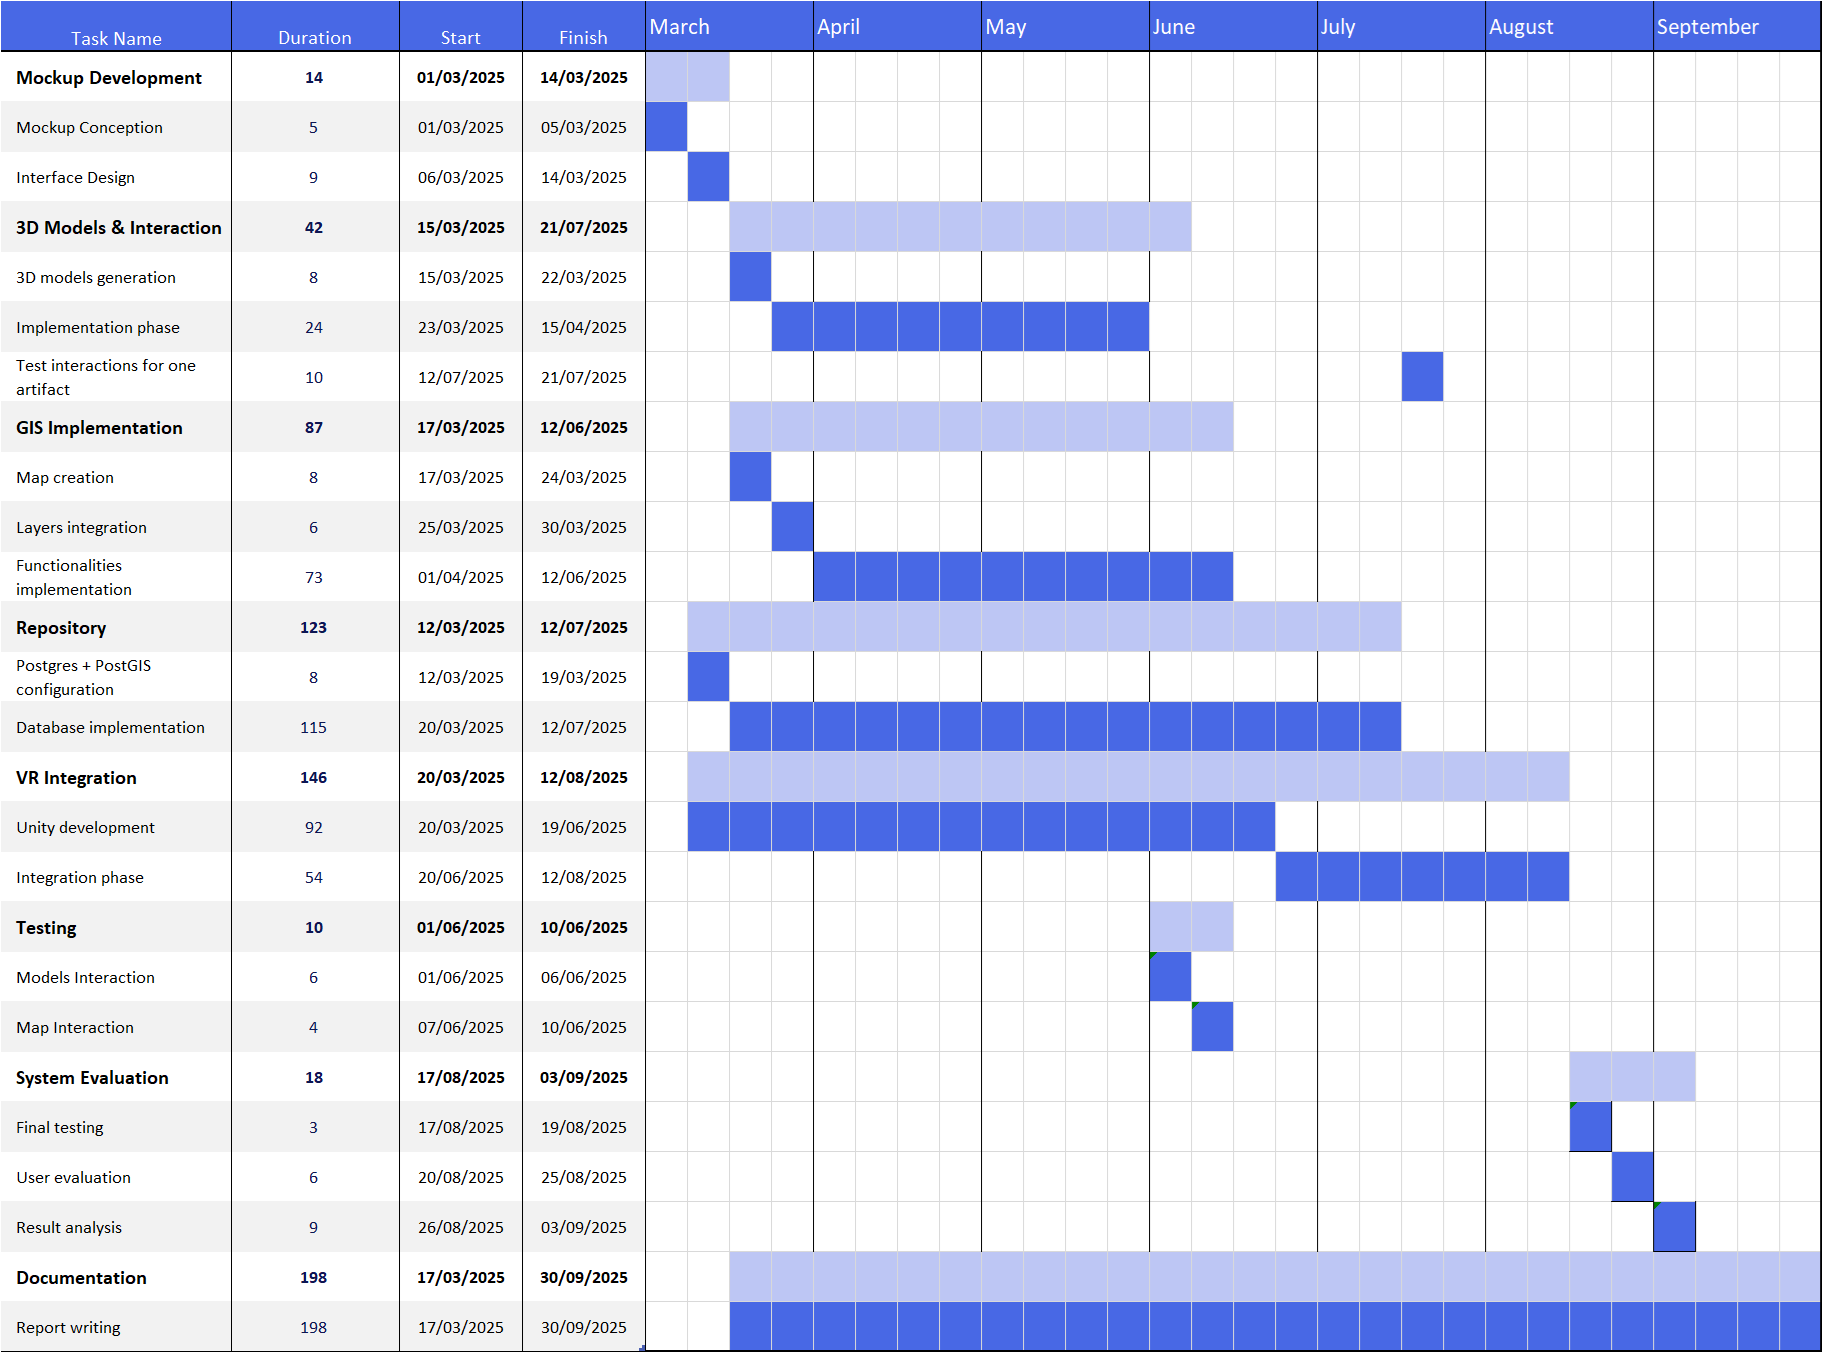
\includegraphics[width=1.0\linewidth]{Gantt_chart}
    \caption{Gantt Chart Representation of the Work Plan.}
    \label{fig:gantt_chart}
  \end{figure}
  \FloatBarrier